\documentclass[a4paper]{article}

\usepackage{fullpage}               % Reduce white space around margins
\usepackage{graphicx}               % For including images
\usepackage{chngcntr}               % For section-wise table/figure counters
\usepackage{caption}                % For specifying figure/table captions and its attributes
\usepackage{geometry}               % For specifying margin sizes
\usepackage{multirow,tabularx}      % For row splits in a table


\date{}                             % Don't print the date
\linespread{1.5}                    % Line spacing = 1.5
\counterwithin{table}{section}      % Count tables per-section
\counterwithin{figure}{section}     % Count figures per-section
\geometry{a4paper, margin=1.00in}

\begin{document}

% Create title page
    \begin{titlepage}
        \vspace*{\fill}
        \begin{center}
            {\huge \bf ECE 521 - Computer Design Techniques \\ Fall 2014 \\ \vspace {8 mm} \\ \LARGE \bf Dynamic Instruction Scheduler \\ \vspace{4 mm} Project Report}
            
            {\vspace{9 mm} \it \large Prepared by \\ \bf \Large Aravindhan Dhanasekaran\\ \bf \large adhanas@ncsu.edu}
        \end{center}
        \vspace*{\fill}
    \end{titlepage}


\pagenumbering{roman}
\newpage
\tableofcontents
\listoffigures
\listoftables
\newpage
\pagenumbering{arabic}


\section{Introduction}
In this project, a dynamic instruction scheduler using Tomasulo's algorithm has been modeled. All stages of Tomasulo algorithm --- instruction fetch, instruction dispatch, instruction issue, instruction execution, results writeback and instruction retirement has been modeled. The dispatch bandwidth and the reservation stations capacity of the scheduler are configurable. 

Also, a multi-level data cache (L1 and L2) with variable cache size and associativity has been modeled.  This cache configuration uses Least Recently Used (LRU) algorithm for aging out older entries.
\section{Important Formulas}
Some of the important formulas that are used to characterize the micro-architecture performance are briefly discussed here.

\subsection{Instructions Per Cycle (IPC)}
As the name suggests, it denotes the average of total number of instructions executed per cycle over a period of time. It is governed by the following formula:

\[IPC = \frac{totalNumInstructions}{totalNumCycles}\]

Though, this formula involves neither the dispatch bandwidth (\textit{n}) nor the scheduling queue size (\textit{s}), both of them affects the overall \textit{IPC} of an architecture. This is explained in more detail in section 5.
\section{Important Definitions and Terms}
Some of the important terms to understand the dynamic instruction scheduler are briefly discussed here.

\subsection{Dispatch Bandwidth}
Dispatch bandwidth (\textit{n}) denotes the maximum number of instructions that can be fetched by the processor in each cycle. In other words, it is the at most number of instructions that a processor can fetch in each cycle. This value plays an important role as it acts as the upper bound for the overall number of instructions that a processor could execute per cycle. 


\subsection{Scheduling Queue Size}
The scheduling queue size (\textit{s}) denotes the number of instructions that can be waiting in the reservation stations (of Tomasulo's algorithm) at any given time. An instruction waits in the reservation station(s) until all of its source operands are available. This value impacts the overall IPC of the processor as the processor cannot fetch new instructions if this queue is full.
\section{Experiments}
Many experiment runs were conducted using different benchmarks to understand how the dispatch bandwidth (n) and scheduling queue size (s) affects the performance of the scheduler. The following sections explains the experiment runs, the scheduler configuration and the results in tables and graphs for two different benchmarks --- gcc and perl.


\subsection{Benchmark gcc}
In this experiment the scheduler is run with different possible configurations (varying values of \textit{n} and \textit{s}) against the gcc benchmark. The dispatch bandwidth is varied in powers of 2 from 1 till 8 and the scheduling queue size is varied from 8 till 256, in powers of 2 again. For each such configuration, the IPC is calculated. The results are tabulated in table \ref{tab:gcc} and the results are plotted as line curves for \textit{s} vs \textit{IPC} for different values of \textit{n} in figure \ref{fig:gcc}.

\begin{table}[htbp]
    \centering
    \noindent \begin{tabular}{|c|c|c|c|c|}
        \hline
        \multirow{2}[4]{*}{\bf Scheduling Queue Size (s) } & \multicolumn{4}{c|}{\bf Instructions Per Cycle (IPC)} \\
        \cline{2-5} & \bf n = 1 & \bf n = 2 & n = 4 & \bf n = 8 \\
        \hline
          8 & 0.99 & 1.88 & 2.67 & 2.82 \\
         16 & 1.00 & 1.99 & 3.54 & 4.54 \\
         32 & 1.00 & 1.99 & 3.90 & 6.48 \\
         64 & 1.00 & 1.99 & 3.97 & 7.52 \\
        128 & 1.00 & 1.99 & 3.97 & 7.83 \\
        256 & 1.00 & 1.99 & 3.97 & 7.83 \\
        512 & 1.00 & 1.99 & 3.97 & 7.83 \\
        \hline
    \end{tabular}
    \captionsetup{justification=centering}
    \caption{Dynamic Scheduler Experiment Data for gcc Benchmark for different \textit{n} and \textit{s} values}
    \label{tab:gcc}
\end{table}

\begin{figure} [htbp]
    \centering
    \noindent {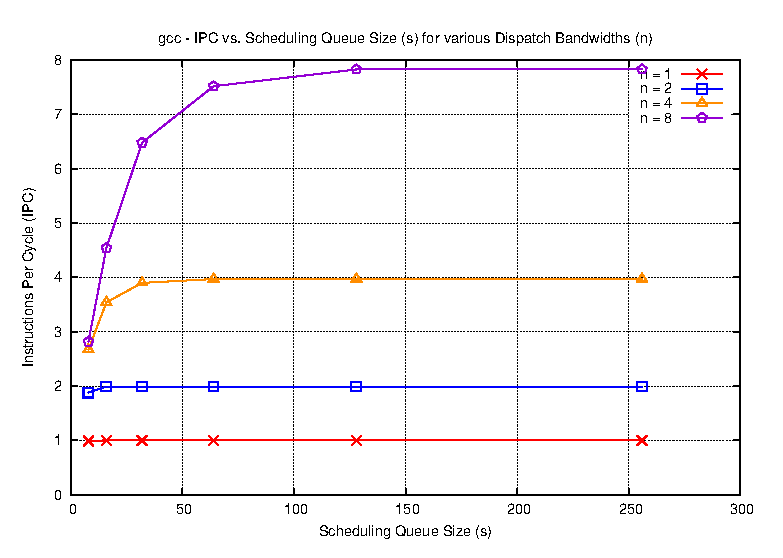
\includegraphics[width=\textwidth, keepaspectratio]{img/gcc.eps}}
    \caption{Scheduling Queue Size vs Instructions Per Cycle for gcc Benchmark}
    \label{fig:gcc}
\end{figure}


\subsection{Benchmark perl}
In this experiment the scheduler is run with different possible configurations (varying values of \textit{n} and \textit{s}) against the perl benchmark. The dispatch bandwidth is varied in powers of 2 from 1 till 8 and the scheduling queue size is varied from 8 till 256, in powers of 2 again. For each such configuration, the IPC is calculated. The results are tabulated in table \ref{tab:perl} and the results are plotted as line curves for \textit{s} vs \textit{IPC} for different values of \textit{n} in figure \ref{fig:perl}.

\begin{table}[htbp]
    \centering
    \noindent \begin{tabular}{|c|c|c|c|c|}
        \hline
        \multirow{2}[4]{*}{\bf Scheduling Queue Size (s) } & \multicolumn{4}{c|}{\bf Instructions Per Cycle (IPC)} \\
        \cline{2-5} & \bf n = 1 & \bf n = 2 & n = 4 & \bf n = 8 \\
        \hline
          8 & 0.98 & 1.68 & 2.18 & 2.28 \\
         16 & 1.00 & 1.89 & 2.91 & 3.37 \\
         32 & 1.00 & 1.98 & 3.68 & 5.18 \\
         64 & 1.00 & 1.98 & 3.91 & 6.95 \\
        128 & 1.00 & 1.98 & 3.94 & 7.61 \\
        256 & 1.00 & 1.98 & 3.94 & 7.75 \\
        512 & 1.00 & 1.98 & 3.94 & 7.75 \\
        \hline
    \end{tabular}
    \captionsetup{justification=centering}
    \caption{Dynamic Scheduler Experiment Data for for perl Benchmark for different \textit{n} and \textit{s} values}
    \label{tab:perl}
\end{table}

\begin{figure} [htbp]
    \centering
    \noindent {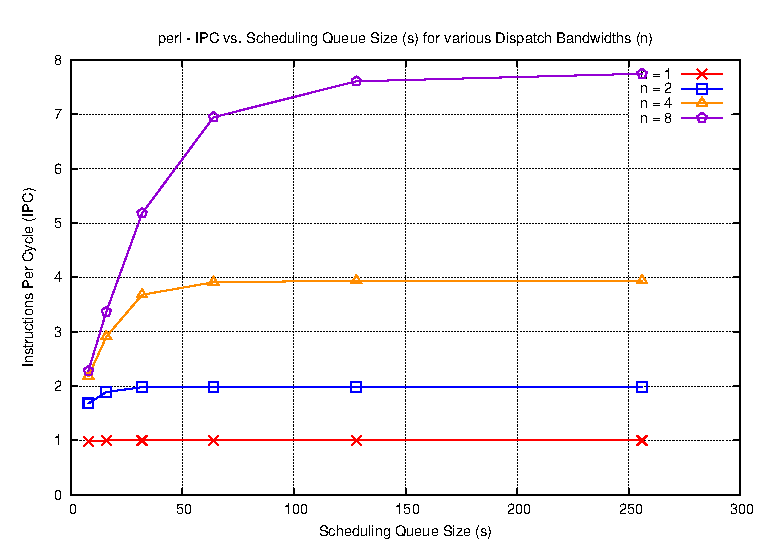
\includegraphics[width=\textwidth, keepaspectratio]{img/perl.eps}}
    \caption{Scheduling Queue Size vs Instructions Per Cycle for perl Benchmark}
    \label{fig:perl}
\end{figure}

\section{Analysis and Trends}
In this section, we analyze the data obtained from the experiment runs that were discussed in section 4. We analyze the data for theoretical correctness, study the relationship between \textit{s}, \textit{n} and \textit{IPC}, and discuss the trends seen amongst different configurations of the same benchmark and finally contrast them with other benchmarks.


\subsection{Theoretical Correctness}
Theoretically speaking, \textit{IPC} should never be greater than the dispatch bandwidth as we can only fetch \textit{n} instructions per cycle, we cannot execute more than \textit{n} instructions per cycle. However, in an ideal case, both \textit{n} and \textit{IPC} should be just the same. This is very evident from the \textit{IPC} values that are shown in tables \ref{tab:gcc} and \ref{tab:perl}. In both the cases, for any value of \textit{n}, \textit{IPC} is less than or equal to that value. 


\subsection{Benchmark Trends}
It can be clearly seen from the figures, \ref{fig:gcc} and \ref{fig:perl} the IPC saturates very quickly for lower values of \textit{n}, given that there is enough buffering to hold all the waiting instructions; i.e., as long as \textit{s} is large enough to hold \textit{n} instructions. Also, the performance of the processor, in terms of the number of cycles that it could execute increases greatly when both \textit{n} and \textit{s} are increased. This could be inferred from the curves for \textit{n} = 8 in figures \ref{fig:gcc} and \ref{fig:perl}.

In order to achieve optimal \textit{IPC}, the dispatch bandwidth should be equal or greater than a certain threshold, in our case, it is 8. This is because, we need a larger window of instructions to find the independent instructions. When \textit{n} is smaller, the window is smaller. Given that most of the dependent instructions are placed adjacent to each to each other, the probability of presence of independent instructions in a smaller window is very less.


\subsection{Benchmark Analysis}
In this section, the results of the experiments are contrasted with various parameters such as ideal IPC value, relationship between \textit{n}, \textit{s} and \textit{IPC}, law of diminishing returns and finally, benchmark comparison.

\subsubsection{Ideal IPC}
It is interesting to note that none of the configurations of the schedulers resulted in an ideal \textit{IPC} of 1, except for cases where the dispatch bandwidth itself is 1. This essentially does not mean ideal, as the final \textit{IPC} is averaged over 2 million values. This actually reflects the real world cases where ideal \textit{IPC} is never reached.

\subsubsection{Law of Diminishing Returns}
It could be inferred from the values in tables \ref{tab:gcc} and \ref{tab:perl} that \textit{IPC} saturates after a threshold and the law of diminishing returns does not apply here, unlike other processor performance attributes such as cache miss rate and branch mis-prediction rate. For gcc benchmark, \textit{IPC} stablizes at \textit{s} = \{16, 16, 64, 128\} for \textit{n} = \{1, 2, 4, 8\} respectively. For perl benchmark, \textit{IPC} stablizes at \textit{s} = \{16, 32, 128, 256\} for \textit{n} = \{1, 2, 4, 8\} respectively. 

\subsubsection{Relationship between \textit{IPC}, \textit{s} \& \textit{n}}
It can be also seen from figures \ref{fig:gcc} and \ref{fig:perl} that \textit{IPC} increases as \textit{s} increases, but this is also influenced by \textit{n}, as the processor cannot finish executing anymore instructions that what it fetches. \textit{IPC} increases when \textit{n} increases too, but it is not entirely independent. It is dependent on \textit{s}; for example in gcc benchmark, for \textit{s} = 8 and \textit{n} = 1, \textit{IPC} is 0.99, but when \textit{n} is increased to 8 with \textit{s} being still at 1, \textit{IPC} is only about 2.82, which is way less than 8. This clearly shows that \textit{IPC} is influenced by \textit{s} more than by what it is influenced by \textit{n}.

\subsubsection{Performance of gcc \& perl Benchmarks}
Also for the same micro-architecture configurations, the \textit{IPC} values are different for gcc and perl benchmarks, with gcc resulting in a slightly better performance. This could be attributed to the instruction distance between interdependent instructions. If iB is dependent on iA and iC is dependent on iB, the time iA takes to finish execution directly impacts the time iB takes and indirectly impacts the wait time for iC. If there are more multi-level interdependent instructions, the performance of the architecture might degrade.

\section{Conclusion}
The key takeaway of this project and the accompanying project report is the understanding of out of order instruction execution using Tomasulo's algorithm for dynamic instruction scheduling. The project and the experimental runs were very instrumental in understanding the the performance characteristics of the instruction scheduler and the factors affecting it.


\end{document}

